
\chapter{Diseño}

% Arquitectura del software, diagramas de clases, diagramas de secuencia

\section{Arquitectura del software}

A continuación muestro un esquema que representa la arquitectura general del software.\newline


\begin{figure}[h]
	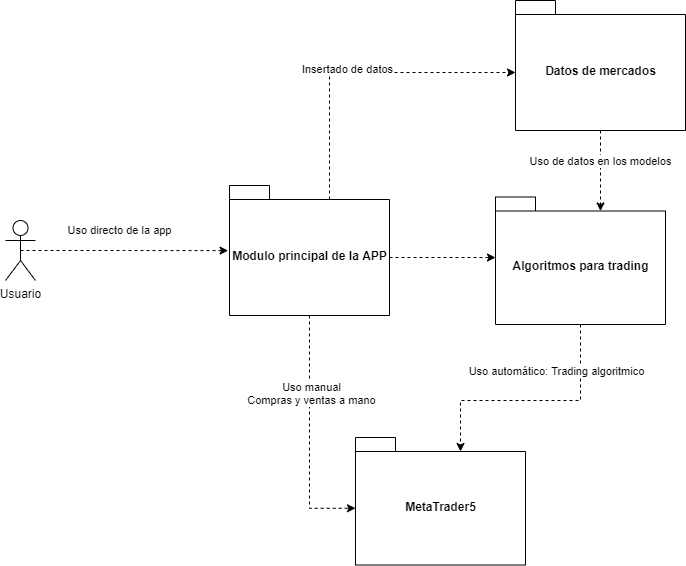
\includegraphics[width=1\textwidth]{imagenes/arquitectura general.png}
	\caption{Arquitectura general del software}
\end{figure}


Como resumen, en el esquema podemos ver cuál es la idea principal del proyecto. El usuario de la aplicación (véase punto \ref{implicados}, segundo implicado) será el que haga un uso directo de la interfaz de la aplicación. A continuación presento cada uno de los módulos con sus funciones y demás utilidades:

\begin{itemize}
	\item \textbf{Módulo principal de la APP}: este módulo se corresponderá con el controlador principal del software. Será usado por el usuario a través de una interfaz escrita en Django y se comunicará con el resto de módulos directamente.
	\item \textbf{Datos de mercados}: este módulo se corresponderá con la base de datos y las operaciones que hagamos con dichos datos (insertado de datos, adaptaciones a cada algoritmo, etc.) Será usado por la interfaz principal de la aplicación y mandará los inputs a los algoritmos.
	\item \textbf{Algoritmos para trading o backend}: se corresponde con el backend o código fuente de la aplicación. Aquí se encontrará cada uno de los algoritmos que usemos para trading algorítmico. Recibe datos de la BBDD y se comunica con el módulo de MetaTrader5 para indicar cada una de las operaciones decididas y obtener información en tiempo real.
	\item \textbf{MetaTrader5}: Módulo externo de la aplicación, se usará para mandar órdenes de operaciones y recibir resultados e información en tiempo real.
\end{itemize}

El software consistirá en una aplicación web con código escrito en Python, usando Django como Framework para la interfaz.

% COMPLETAR CON MAS DETALLES DE HERRAMIENTAS

\section{Primer diseño de la interfaz}

La página web principal mostrará un menú con distintos botones que implementan funcionalidades diferentes. Previo a este menú tendremos un formulario para identificarnos como usuarios de la aplicación. A ambos lados del menú principal y durante todas las vistas de la APP tendremos hiperenlaces con accesos directos a distintas funcionalidades de la aplicación. A continuación muestro una serie de borradores con diseños de cada una de las secciones de la interfaz.\newline

En este primer diseño que muestro en la siguiente imagen, se puede ver el menú principal de la aplicación.\newline

\begin{figure}[h] \label{menu_principal}
	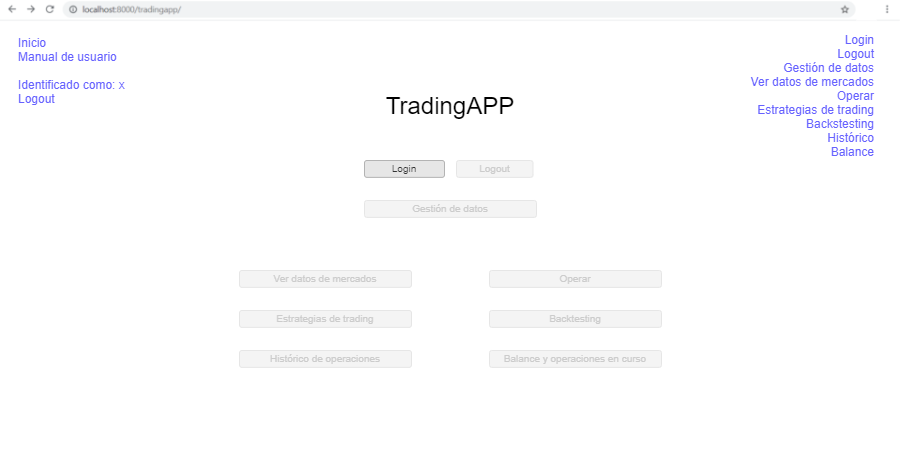
\includegraphics[width=1.2\textwidth]{imagenes/menu_principal}
	\caption{Primer diseño del menú principal de la APP}
\end{figure}

En la imagen mostrada vemos los siguientes botones: \textit{Login}, \textit{Logout}, \textit{Gestión de datos},\textit{ Mi perfil}, \textit{Ver datos de mercados}, \textit{Operar}, \textit{Estrategias de trading}, \textit{Backtesting}, \textit{Histórico de operaciones} y \textit{Balance y operaciones en curso}. En los puntos siguientes explico qué realizaría cada botón y con qué parte del software conectaría.\newline

\begin{itemize}
	\item \textbf{Login}: permite conectar a nuestra cuenta de MetaTrader5, comercial o demo. Véase la siguiente figura. \textit{\textbf{Referencia}: login, RF-1.1.}
	\item \textbf{Logout}: permite cerrar la sesión iniciada anteriormente con el menú de Login. Este botón no estará habilitado hasta que hayamos iniciado sesión. \textit{\textbf{Referencia}: login, RF-1.1.}
	\item \textbf{Gestión de datos}: permite el insertado y procesado de datos de mercado. El usuario podrá a través del menú correspondiente introducir datos al módulo que se encarga de gestionar la BBDD. Al ser un módulo totalmente independiente del módulo de MetaTrader5, no será necesario haber iniciado sesión anteriormente. \textit{\textbf{Referencia}: procesado de datos, RF-2.}
	\item \textbf{Mi perfil}: permite indicar la información del bróker usado. En este menú indicamos información sobre comisiones u otros parámetros.
	\item \textbf{Ver datos de mercados}: permite ver datos de precios de un mercado elegido. Se permite ver datos en un marco de tiempo específico, en rango y de mercados específicos. \textit{\textbf{Referencia}: visualización de datos, RF-3.}
	\item \textbf{Operar}: lleva al usuario a un menú donde podrá operar manualmente, es decir, gestionando las operaciones abiertas y/o abriendo nuevas; o usando el trading algorítmico. \textit{\textbf{Referencia}: operar manualmente, RF-4; trading algorítmico, RF-5.} 
	\item \textbf{Estrategias de trading}: lleva a un menú en el que se puede obtener información de cada una de las estrategias de trading así como elegir una para que sea usada en las próximas operaciones. \textit{\textbf{Referencia}: trading algorítmico, RF-5.} 
	\item \textbf{Backtesting}: menú similar a Operar. En este caso el usuario podrá iniciar operaciones manualmente o usando trading algorítmico a partir de una fecha anterior a la actual, simulando el transcurso del tiempo. \textit{\textbf{Referencia}: backtesting, RF-6.} 
	\item \textbf{Histórico de operaciones}: permite al usuario ver un resumen del histórico de operaciones realizadas. \textit{\textbf{Referencia}: información de operaciones, RF-1.3.} 
	\item \textbf{Balance y operaciones en curso}: permite al usuario ver el capital disponible, así como un balance a tiempo real de pérdidas y ganancias y el resumen de las operaciones en curso. \textit{\textbf{Referencia}: capital disponible, RF-1.2; información de operaciones, RF-1.3.} 
\end{itemize}

A continuación muestro una imagen de lo que sería el menú de \textbf{Login}. En este menú se introducirán Login, Contraseña y Servidor para que nuestra aplicación inicie sesión en la cuenta demo o comercial de MetaTrader5.\newline

\begin{figure}[h]
	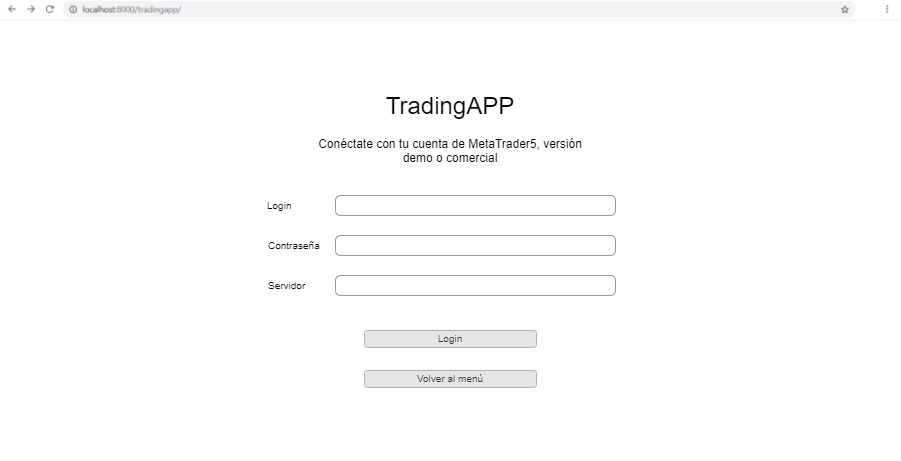
\includegraphics[width=1.2\textwidth]{imagenes/menu_login}
	\caption{Primer diseño del formulario de login en \textit{MT5}}
\end{figure}

Una vez estemos conectados en la cuenta de MT5, nuestro menú principal mostrará disponibles las funcionalidades que en la figura \ref{menu_principal} no estaban habilitadas. Dichas funcionalidades dependen directamente del módulo de MT5, por lo que necesitan de conexión a la cuenta. \newline

\begin{figure}[h]
	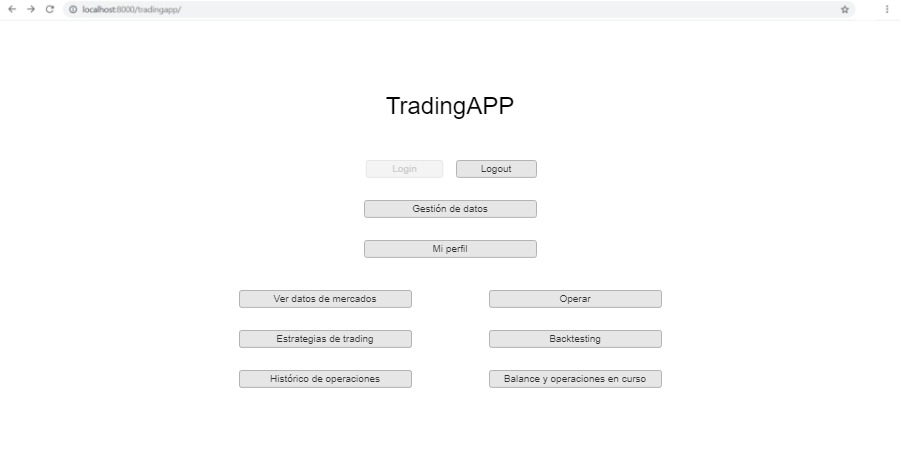
\includegraphics[width=1.2\textwidth]{imagenes/menu_principal_logued}
	\caption{Primer diseño del menú principal (usuario identificado en \textit{MT5}) }
\end{figure}



